%----------------------------------------------------------------------------------------
%	SECTION 1.1
%----------------------------------------------------------------------------------------

\section{Topological Spaces.}

\begin{definition}
    A \textbf{topology} on a set $X$ is a collection  $\Tc$ of subsets of  $X$ such that:
        \begin{enumerate}
            \item[(1)] $\emptyset \in \Tc$ and $X \in \Tc$

            \item[(2)] For any collection $\{U_{\alpha}\}$ of subsets of $X$,
                $\bigcup_{\alpha}{U_{\alpha}} \in \Tc$.

            \item[(3)]  For any finite collection $\{U_i\}_{i=1}^{n}$ of subsets of $X$,
                $\bigcap_{i=1}^{n}{U_i} \in \Tc$.
        \end{enumerate}
        We call the pair $(X,\Tc)$ a \textbf{topological space}, and we call the elements
        of  $\Tc$ \textbf{open sets}.
\end{definition}

\begin{example}
    \begin{enumerate}
        \item[(1)] Let $X$ be any set, the collection of all subsets of  $X$,
            $2^X$ is a topology on $X$, which we call the \textbf{discrete
            topology}. We call the topology $\Tc= \{\emptyset, X\}$ the
            \textbf{indiscrete topology}.

        \item[(2)] The set of three points $\{a, b, c\}$ has the  $9$ following
            topologies
            in figure \ref{fig1.1}.
            \begin{figure}[h]
                \centering
                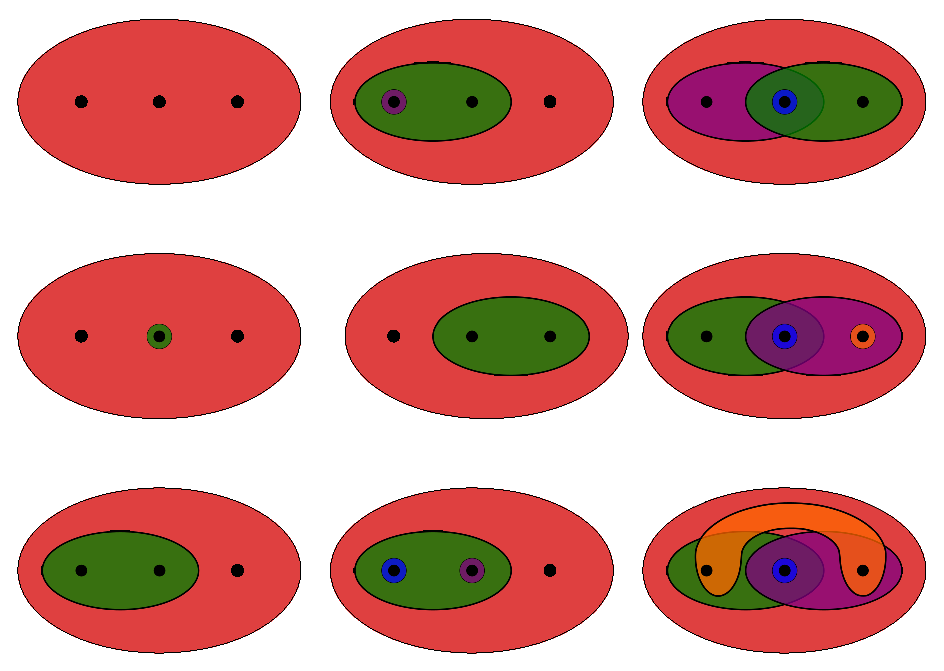
\includegraphics[scale = 0.5]{Figures/Chapter1/three_point_topology.eps}
                \caption{The Topologies on $\{a, b, c\}$.}
                \label{fig1.1}
            \end{figure}

        \item[(3)] Let $X$ be any set, and let  $\Tc_f=\{U \subseteq X: \com{X}{U}
                \text{ is finite, or } \com{X}{U}=X\}$. Then  $\Tc_f$ is a
                topology and called the \textbf{finite complement topology}.

        \item[(4)] Let $X$ be any set, and let  $\Tc_c=\{U \subseteq X: \com{X}{U}
                \text{ is countable, or } \com{X}{U}=X\}$. Then  $\Tc_c$ is a
                topology on $X$ called the \textbf{countable complement
                topology}.

            \item[(5)] Let $X$ be any set and consider the collection
                $\Tc_\infty=\{U \subseteq X : \com{{X}}{U}=\emptyset,
                \com{X}{U}=X, \text{ or } \com{X}{U} \text{ is infinite}\}$.
                Certainly, we have that $\emptyset,X \in \Tc_\infty$ as
                $\com{X}{X}=\emptyset$ and $\com{X}{\emptyset}=X$.

                However, if $X=\R$, and we have the sets $(0,1)$, and
                $(-\infty,0) \cup (1, \infty)$, then
                $\com{\R}{(0,1)}=(-\infty,0] \cup [1,\infty)$, and
                $\com{\R}{(-\infty,0) \cup (1, \infty)}=[0,1]$, both of which
                are infinte, but, $[0,1] \cap ((-\infty,0] \cup
                [1,\infty))=\{0,1\}$, which is finite. So it is not true in
                general that the collection $\Tc_\infty$ is a topology.
    \end{enumerate}
\end{example}

\begin{lemma}\label{1.1.1}
    Let $X$ be a topological space. If  $A \subseteq X$ is such that for each
    $x \in A$, there exists an open set  $U$ with  $x \in U \subseteq A$, then
    $A$ is also open in  $X$.
\end{lemma}
\begin{proof}
    We have that for each $x \in A$, there is an open set  $U_a$ such that  $x
    \in U_x \subseteq A$. Now, let  $U=\bigcup_{x \in A}{U_x}$, which is open in
    $X$ by definition. Then, we have $U \subseteq A$ by hypothesis; moreover,
    since  $x \in A$ implies  $x \in U_x$, then  $x \in U$. This makes
    $A \subseteq U$, so  $A=U$.
\end{proof}

\begin{definition}
    Let $X$ be a set, and let $\Tc$ and  $\Tc'$ be topologies on  $X$. We say that
    $\Tc$ is  \textbf{coarser} than $\Tc'$, and $\Tc'$ \textbf{finer} than $\Tc$ if
    $\Tc \subseteq \Tc'$.
    If two topologies are either coarser, or finer than each other, we call them
    \textbf{comparable}.
\end{definition}

\begin{example}
    The topologies $\Tc_f$ and  $\Tc_c$ are comparable, and we see that  $\Tc_f
    \subseteq \Tc_c$, so $\Tc_f$ is coarser than  $\Tc_c$, and  $\Tc_c$ is finer than
    $\Tc_f$.
\end{example}

\begin{lemma}\label{1.1.2}
    If $\{Tc_\alpha\}$ is a collection of topologies on a set $X$, then the
    intersection of all  $\Tc_\alpha$,  $\bigcap{T_\alpha}$ is also a topology
    on $X$.
\end{lemma}
\begin{proof}
    Let $\Tc=\bigcap{\Tc_\alpha}$. We have that $\emptyset, X \in \Tc_\alpha$
    for each  $\alpha$, so that  $\emptyset, X \in \Tc$.

    Now let  $\{U_\alpha\}$ be a collection of open sets such that $U_\alpha \in
    \Tc_\alpha$ for each  $\alpha$. Then  $U_\alpha \in \Tc$, for each
    $\alpha$, so that  $\bigcup{U_\alpha} \in \Tc$. Lastly, take a finite
    subcollection $\{U_i\}_{i=1}^n$ of $\{U_\alpha\}$, then
    $\bigcap_{i=1}^n{U_i} \in \Tc$ by similar reasoning.
\end{proof}

\begin{example}\label{1.3}
    If $X$ is any set, and  $\{Tc_\alpha\}$ is a collection of topologies in
    $X$, it is not in general true that  $\bigcup{\Tc_\alpha}$ is also a
    topology on $X$. Consider the  $9$ topologies on the set  $X=\{a,b,c\}$ in
    the preceding examples. Let $\Tc_1=\{\emptyset, \{a\}, \{a,b\},X\}$,
    $\Tc_2=\{\emptyset, \{a,b\}, \{b\}, \{b,c\}, \{c\}, X\}$ , and let
    $\Tc_3=\Tc_1 \cup \Tc_2$. The sets $\{a\}$ and $\{c\}$ have union $\{a.c\}$,
    however, $\{a,c\} \notin \Tc_3$.
\end{example}
